
% Prepare for svenska tecken
%\usepackage[T1]{fontenc}
\usepackage[swedish]{babel}
\usepackage{icomma}
\usepackage{lmodern}
\usepackage[numbered]{bookmark}
%\usepackage[]{geometry}
\addto\captionsswedish{\renewcommand{\figurename}{Bild}}
\usepackage{amsmath}
\usepackage{fancyhdr}
\usepackage{wrapfig}
\usepackage{caption}
\usepackage{framed}
%\usepackage[fulladjust]{marginnote}
\usepackage{color}
%\newcommand{\hilight}[1]{\colorbox{yellow}{#1}}
%\usepackage[toctitles]{titlesec}
%\usepackage{hyperref}
\usepackage{siunitx}
\sisetup{exponent-product = \cdot, 
	output-product = \cdot,
	output-decimal-marker = {,}}
\hypersetup{
    pdftitle={KonCEPT för amatörradiocertifikat},
    pdfauthor={Föreningen Sveriges Sändareamatörer},
    pdfkeywords={Sveriges Sändareamatörer, SSA, amatörradio},
    pdflang={sv},
    colorlinks,
    citecolor=black,
    filecolor=black,
    linkcolor=black,
    urlcolor=black
}
\usepackage{stmaryrd} % För symbolen \boxbox, kräver paketet texlive-math-extra
\usepackage{gensymb}

\clubpenalty=9999
\widowpenalty=9999
\brokenpenalty=4999

\usepackage[europeanvoltages,europeancurrents,europeanresistors,cuteinductors,smartlabels]{circuitikz}
\usepackage[framemethod=TikZ]{mdframed}

\mdfdefinestyle{FactBox}{%
    linecolor=blue,
    outerlinewidth=2pt,
    roundcorner=20pt,
    innertopmargin=\baselineskip,
    innerbottommargin=\baselineskip,
    innerrightmargin=20pt,
    innerleftmargin=20pt,
    backgroundcolor=gray!50!white}

\newcommand{\infobox}[1]{
\begin{wrapfigure}{r}{0.5\textwidth}
  \begin{mdframed}[style=FactBox]
#1
  \end{mdframed}
\end{wrapfigure}
}

% Prepare for tables
\usepackage{multirow}
\usepackage{longtable}

% Prepare for lists
\usepackage{enumitem}

% Prepare for graphics
\usepackage{xspace,graphicx}

\raggedbottom

% Prepare for version handling
\usepackage{xstring}
\usepackage{catchfile}
\CatchFileDef{\HEAD}{.git/refs/heads/master}{}
\newcommand{\gitrevision}{%
  \StrLeft{\HEAD}{7}%
}
\CatchFileDef{\VERSION}{VERSION.txt}{}
\newcommand{\revision}{%
  \VERSION \gitrevision%
}

%% Frontpage bacground
\usepackage{eso-pic}
\newcommand\BackgroundPic{%
\put(0,0){%
\parbox[b][\paperheight]{\paperwidth}{%
\vfill
\centering
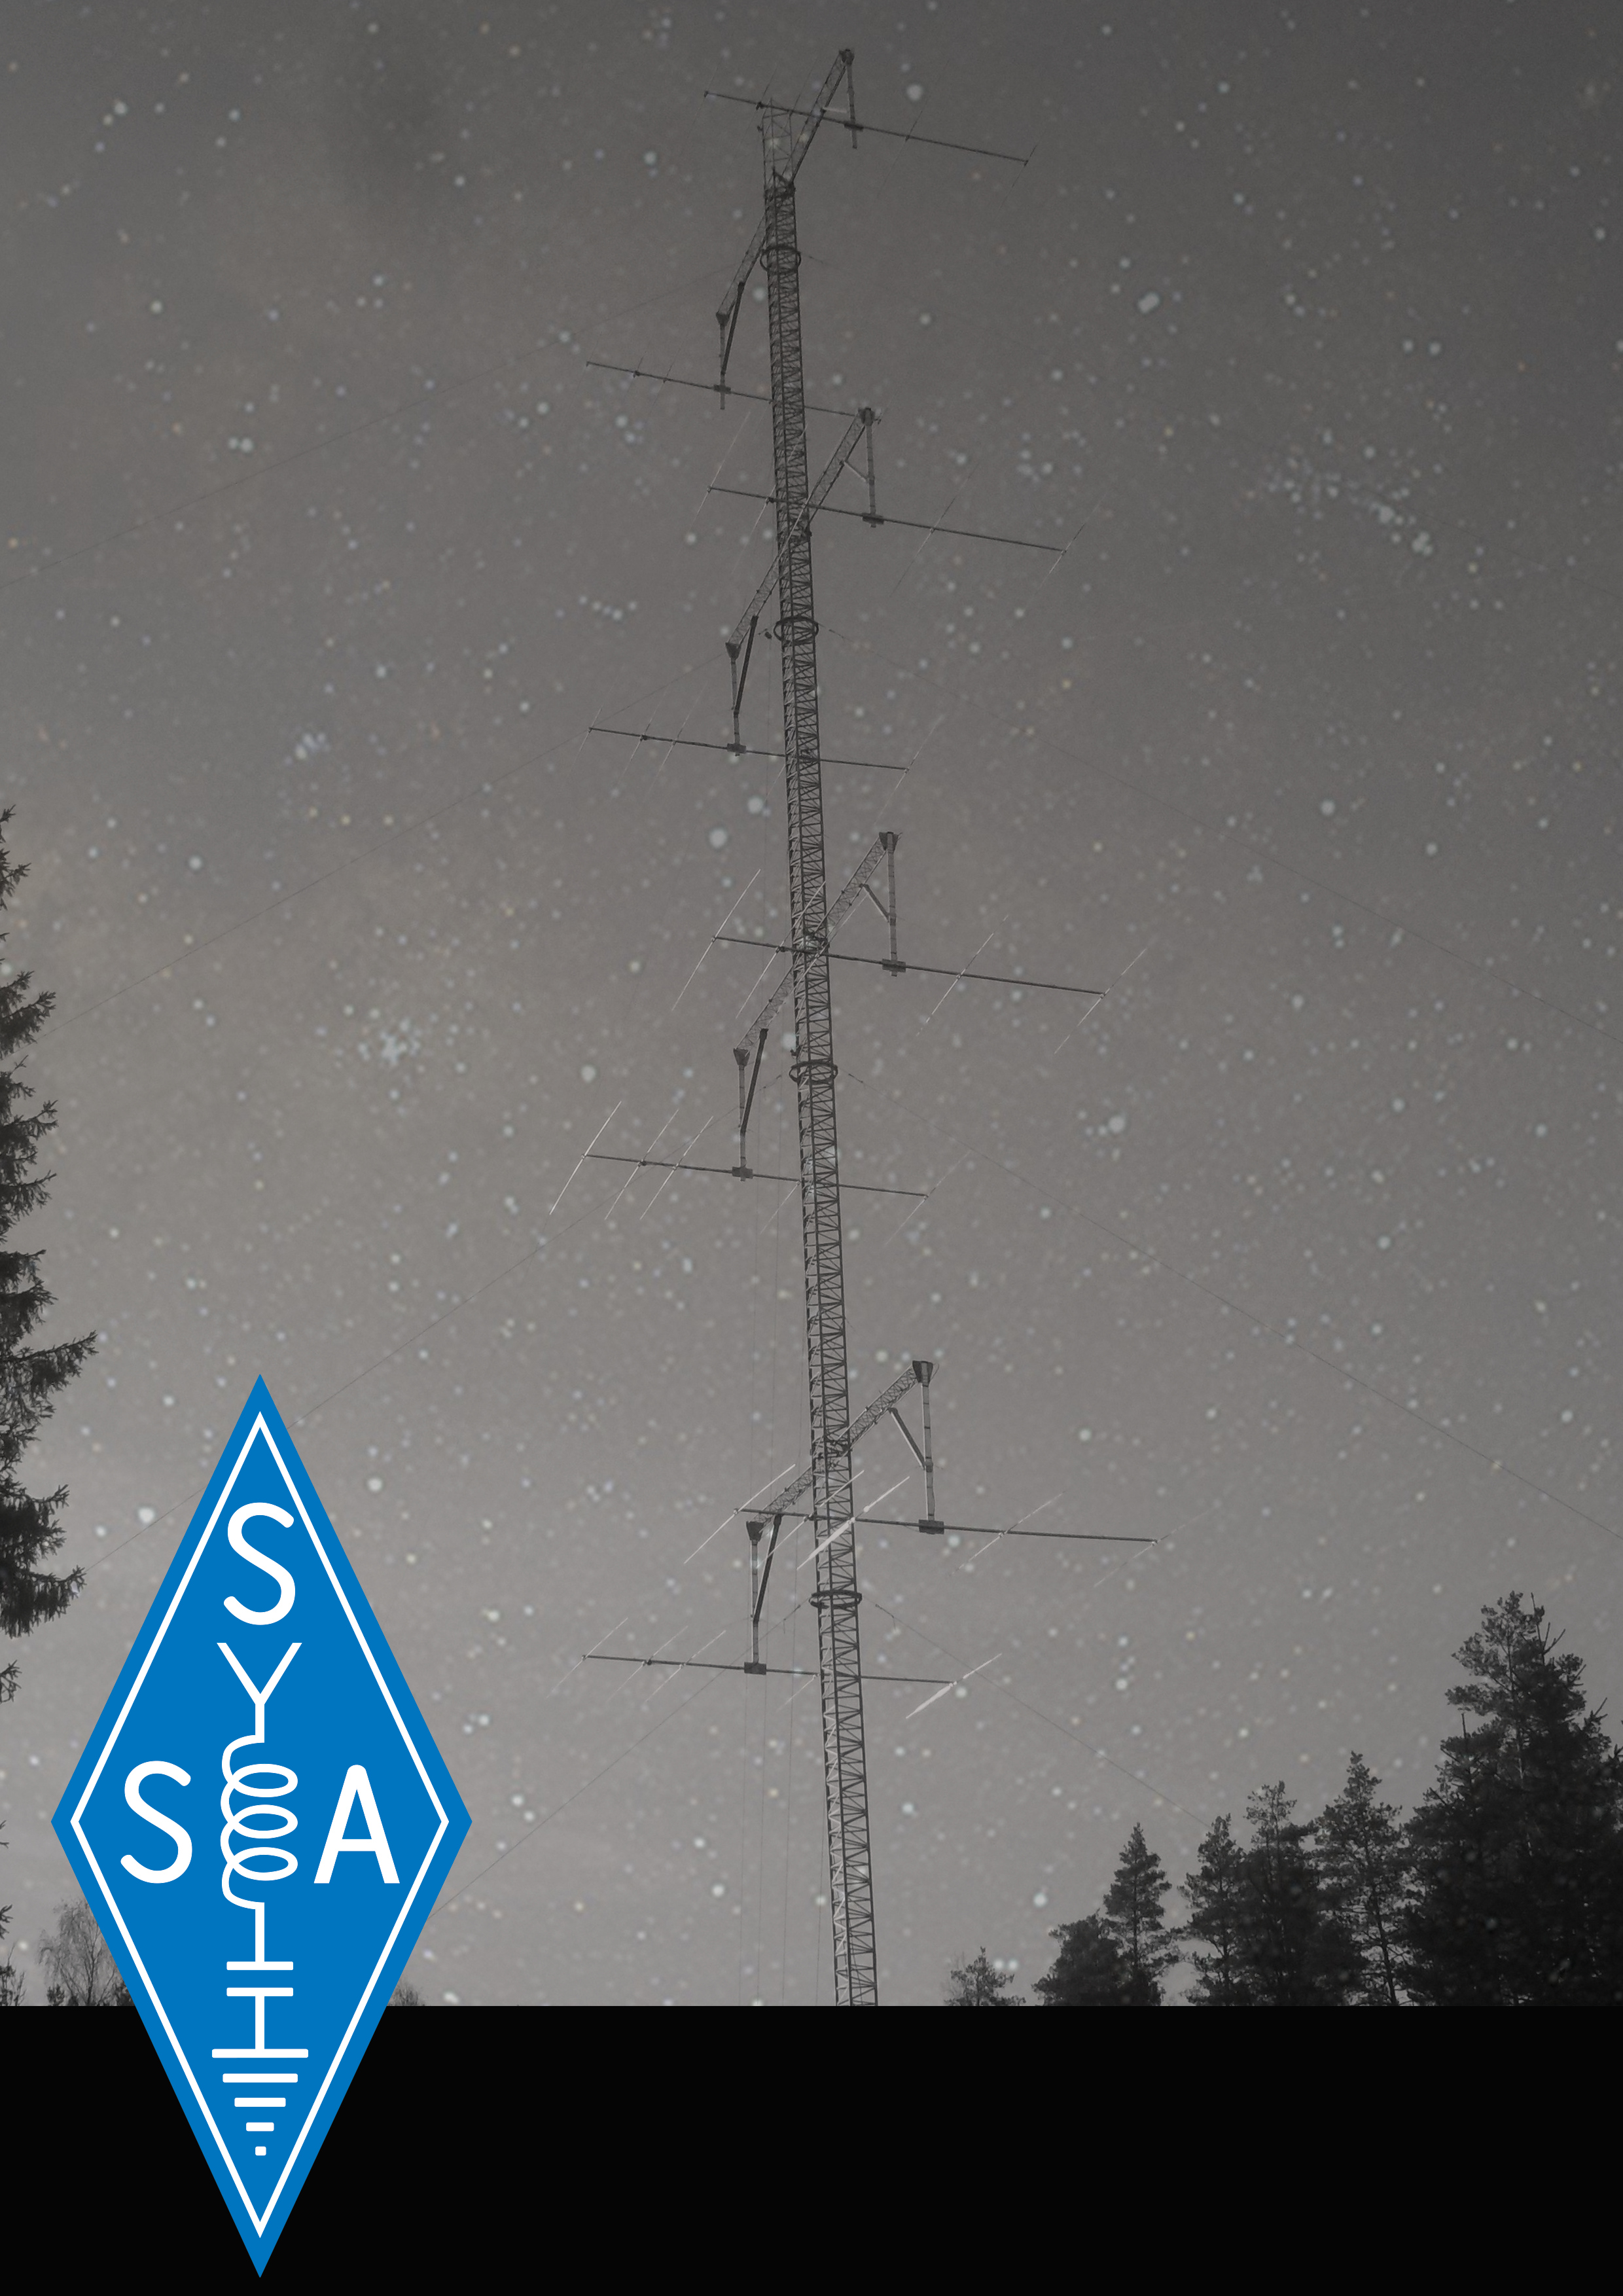
\includegraphics[width=\paperwidth,height=\paperheight,%
keepaspectratio]{images/koncept-front.jpg}%
\vfill
}}}


\newcommand\Backgroundtwo{%
\put(0,0){%
\parbox[b][\paperheight]{\paperwidth}{%
\vfill
\centering
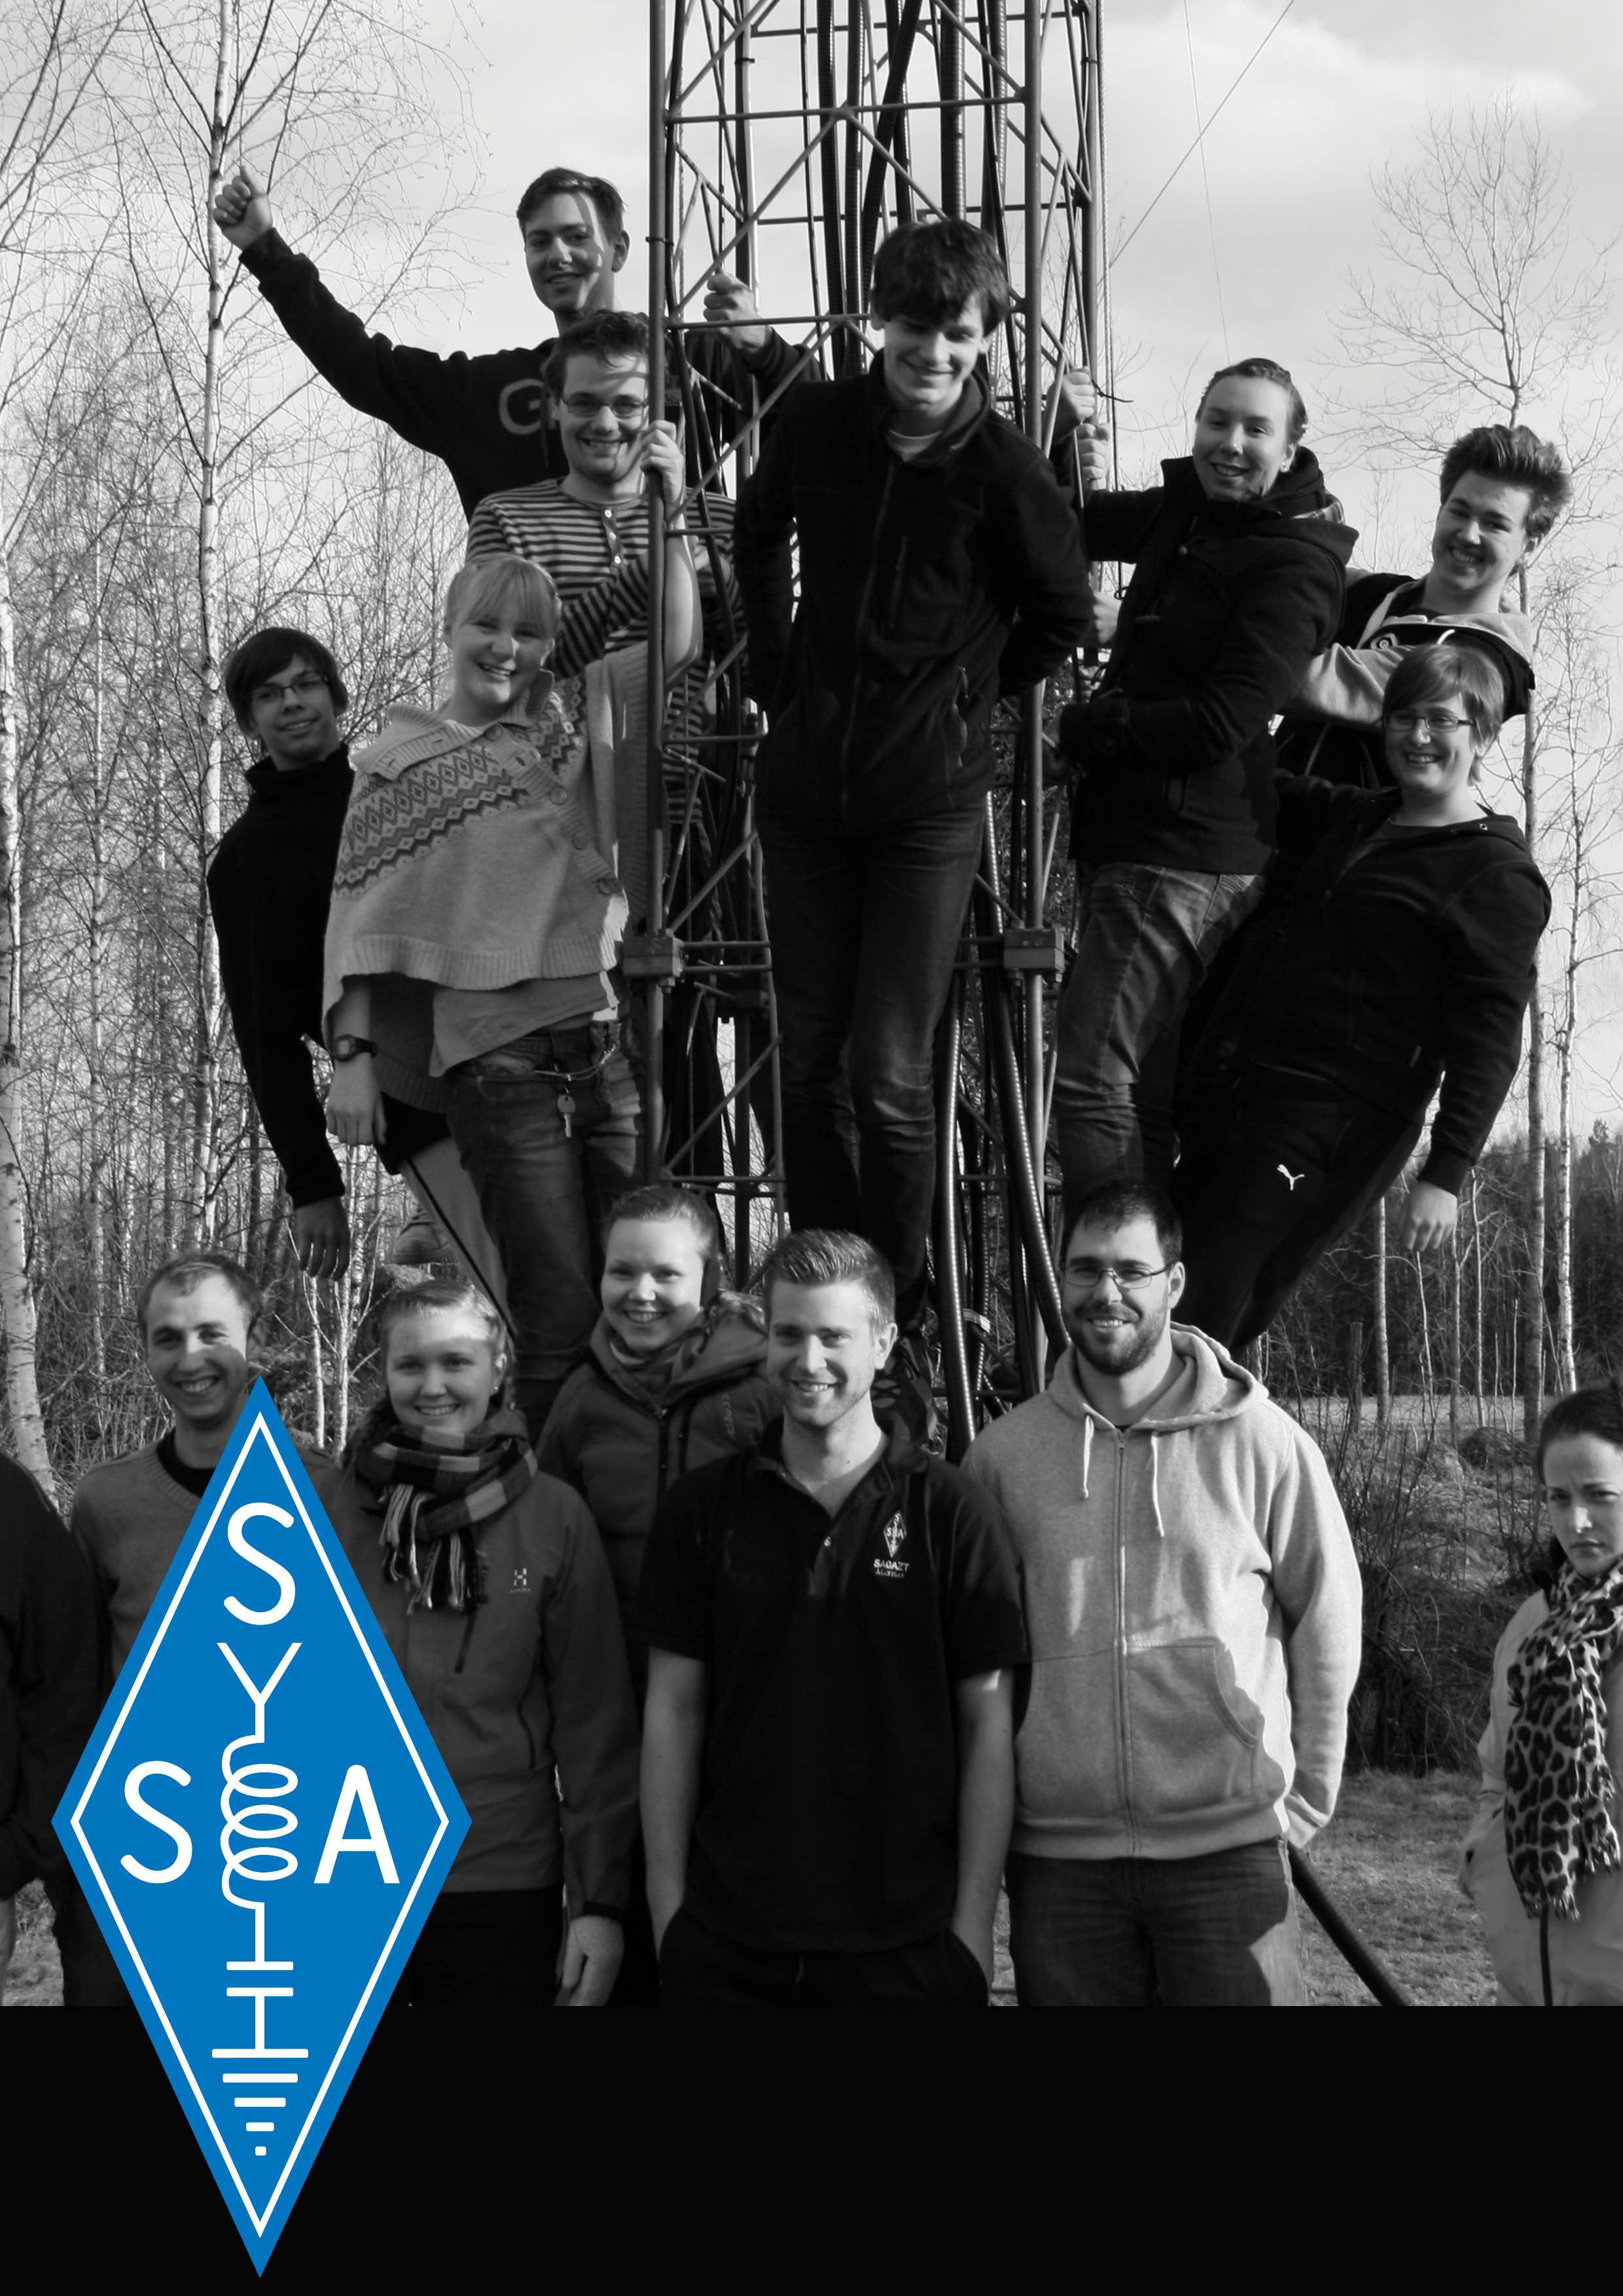
\includegraphics[width=\paperwidth,height=\paperheight,%
keepaspectratio]{images/koncept-larobok-front.jpg}%
\vfill
}}}



\newcommand\BackgroundPicLast{%
\put(0,0){%
\parbox[b][\paperheight]{\paperwidth}{%
\vfill
\centering

\includegraphics[width=\paperwidth,height=\paperheight,%
keepaspectratio]{images/koncept-back.pdf}%
\vfill
}}}
